\subsection{SOlUCIÓN 4}

\subsubsection{Actividad 1 lab 4}
%*********************
\begin{frame}{}

\pgfdeclareimage[width=\paperwidth,height=\paperheight]{bg}{imagenes/fondo_seccion}
\setbeamertemplate{background}{\pgfuseimage{bg}}

\definecolor{greenU}{RGB}{212,202,72}
\setbeamercolor{block body}{fg=Black,bg=greenU}
\begin{block}{}
	\centering
	\vspace{1mm}
	\large{\textit{solucion lab 4 actividad 1}}
	\vspace{1mm}
\end{block}
\end{frame}

%------------------------------------------------------------------------------- 

\begin{frame}{"¿Como observar la constelación de una modulación ASK?"}
\begin{flushleft}
En estos tipos de modulación digital se pueden observar los diagramas de constelación de la siguiente manera:
\end{flushleft}
\begin{itemize}
  \item {Modulación ASK}
  \item {Modulación FSK}
  \item {Modulación PSK}
\end{itemize}
\end{frame}
%-------------------------------------------------------------------------------

\begin{frame}{"Tipos de Modulaciones ASK"}
\begin{flushleft}
\begin{itemize}
\item {
La  Modulación por desplazamiento de amplitud (ASK) es un esquema de modulación digital en el que la amplitud de la onda portadora se cambia con respecto a la señal de información, manteniendo la fase y la frecuencia de constantes. }
\end{itemize}
\begin{itemize}
\item {
La modulación por desplazamiento de frecuencia (FSK)  es un tipo de modulación de frecuencia cuya señal modulante es un flujo de pulsos binarios que varía entre valores predeterminados. }
\end{itemize}
\begin{itemize}
\item {
La modulación por desplazamiento de fase (PSK) es un tipo de modulación angular que consiste en hacer variar la fase de la portadora entre un número de valores discretos. }
\end{itemize}
\end{flushleft}
\end{frame}
%-------------------------------------------------------------------------------

\begin{frame}{"Constelación PSK"}
\begin{flushleft}
Conectamos el wx GUI constellation Sink a la modulacion ASK Y FSK obtendremos la siguiente grafica
\end{flushleft}
\begin{figure}
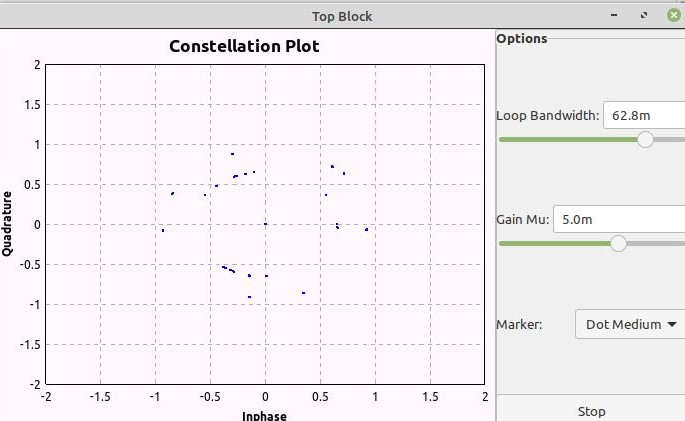
\includegraphics[width=0.8\textwidth]{soluciones/actividad-4-1/pdf/01.pdf}
\end{figure}
\end{frame}

%-------------------------------------------------------------------------------

\begin{frame}{"Constelación ASK Y FSK"}
\begin{flushleft}
Conectamos el wx GUI constellation Sink a la modulacion PSK obtendremos la siguiente grafica
\end{flushleft}
\begin{figure}
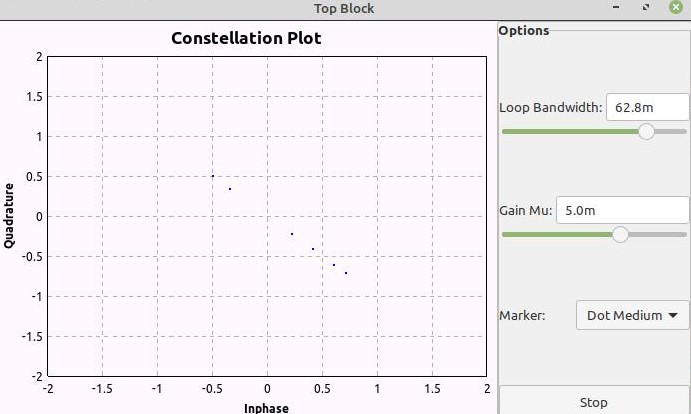
\includegraphics[width=0.8\textwidth]{soluciones/actividad-4-1/pdf/02.pdf}
\end{figure}
\end{frame}